\documentclass[11pt]{article}
\usepackage[top=1cm,bottom=2.50cm,left=2.0cm,right=2.0cm]{geometry}
\usepackage{amsmath}
\usepackage{amssymb}
\usepackage{graphicx}
\usepackage{amssymb}
\usepackage{enumitem}
\usepackage{multicol}

\graphicspath{ {../figures/} }
\renewcommand{\vec}[1]{\mathbf{#1}}
\newcommand{\R}{\rm I\!R}
\newcommand{\comment}[1]{}
\font\titlefont=cmr12 at 15pt

\begin{document}
\author{Gerardo F. Salazar}
\title{\vspace{-.5cm}{\textbf{ \Large PGA Tour Driving Distance Switchpoint Analysis}}\\[5pt]
\vspace{-2.0ex}}
\date{}
\maketitle
\vspace{-1cm}

\begin{multicols}{2}
\section{Purpose}
The players on the PGA Tour represent the most elite athletes in the sport of golf. As such, their performance far exceeds that of the average golfer. The most apparent example of this is the average driving distance of PGA Tour players. While the average driving distance of an amateur golfer is about 220 yards, modern PGA Tour pros regularly average over 300 yards. Over the last two decades, an increasing amount of golf clubs have had to renovate their courses to make them challenging enough for Tour level play. These renovations often cost millions of dollars and take many months to complete. This has recently sparked a discussion around sustainability and the idea of mitigating the trend of increasing Tour players' distance. The purpose of this analysis is thus to characterize the distribution and evolution of average driving distances on Tour so as to provide context and insight for domain-level stakeholders.
\section{Data}
\subsection{Extraction}
The parent data source for this analysis is \textbf{pga\_data\_historical.csv}. The target data for this analysis is the average driving distance statistic, averaged over all players in a given tournament, for all tournaments, arranged in chronological order. The \textit{average of the average} driving distances statistic for a tournament is herein referred to as the ``average driving distance'' of the tournament for simplicity. The result is a time-series of 1720 data points representing the evolution of the average driving distance on the PGA Tour over the last four decades. The data is extracted, transformed, and saved with the \textbf{driving-data.py} script.
\subsection{Considerations}
The average driving distance statistic for each player is calculated by taking the average of the player's driving distance on two fixed holes facing in opposite directions. Taking the measurements on holes facing in opposing directions mitigates the effects of the wind on the measured values. 
\par The number of players per tournament ranges from 132 to 156. The set of players at each tournament can be considered a random sample of the total population of players eligible for each event (typically this implies holding a PGA Tour card, although some tournaments, like the four majors, are more restrictive).
\par There may exist some sparse periodicity in the data given that most tournaments are typically played at the same course year after year. There are exceptions to this (i.e. some of the majors) as well as periodic changes to the Tour schedule that disrupt this periodicity. Compounding this with the significant effects of weather conditions on playing outcomes and the long period between playing the same course twice we ignore any correlation effects and assume the average driving distance of each tournament to be an i.i.d draw from a parent distribution. By application of the Central Limit Theorem to the samples of average driving distance we can assume that the parent distribution is a Normal distribution.
\section{Model/Analysis}
The goal of the analysis is to describe the distribution of driving distances This is a natural setting for applying Bayesian Inference and probabilistic programming. I consider the following \textit{switchpoint} model for the underlying data generating process
$$ \tau \sim \text{DiscreteUniform}(0,1720)$$
$$ \mu = \begin{cases}
    \mu_1 & t < \tau\\
    \mu_2 & t \geq \tau
\end{cases}$$
$$ \sigma = \begin{cases}
    \sigma_1 & t < \tau\\
    \sigma_2 & t \geq \tau
\end{cases}$$
$$ \mu_i \sim \text{Normal}(280,20)$$
$$ \sigma_i \sim \text{Half-Normal}(40)$$
$$ x_t \sim \text{Normal}(\mu, \sigma)$$
\end{multicols}
\begin{center}
    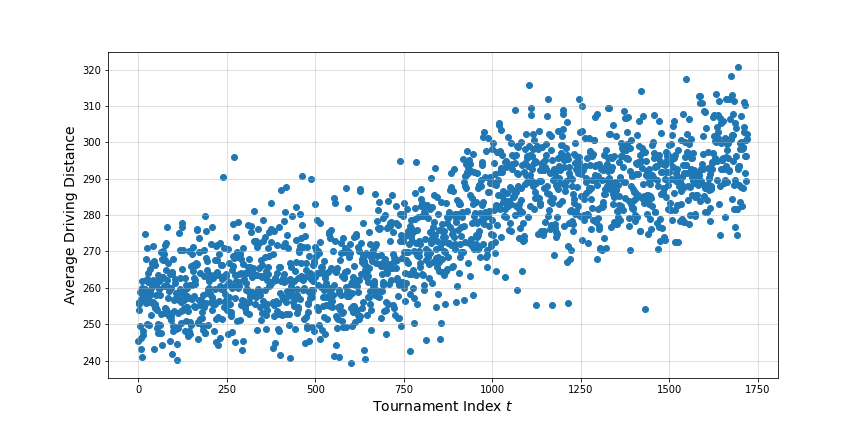
\includegraphics[scale=0.5]{/home/gerardo/Desktop/Projects/PGA-Analysis/reports/figures/average-driving-distance-raw.png}\\
    Figure 1: Average Driving Distance as a function of Tournament Index, $t$. The trend appears to begin relatively flat, trend upwards between $t=750$ and $t=1000$, and then flatten out again. 
\end{center}
\begin{multicols}{2}
In this model, $t$ indexes time. This model represents the belief that there exists a \textit{switchpoint} $\tau$ which causes a shift in the parameters of the distribution which govern the data. The governing distribution is taken to be Normal following the discussion in Section 2.2. The prior on $\tau$ is uniform over the domain of the samples so as not to inject any bias about where the switchpoint might occur. The hyperpriors $\mu_i$ and $\sigma_i$ encode domain knowledge about the parameters of the governing distribution and act serve to provide a warm start for where the sampler should look. The hyperprior on $\sigma_i$ is taken to be a Half-Normal distribution to enforce the fact that it is strictly positive. Driving distances are also strictly positive, but in practice a hyperprior encoding a reasonable estimate for the means prevents the sampler from wandering out of the support of the data and corrupting the results. Inference is preformed with the default No-U-Turn Sampler implementation of PyMC3 which prodcues four traces for each parameter. The \textbf{driving-distance-sp-pymc3.py} script performs inference on the model and outputs the posterior traces. 
\end{multicols}

\begin{multicols*}{2}
\section{Results}
The traces of the sampler for each parameter are shown in Figure 2. 
\section{Conclusion}
    
\end{multicols*}
\begin{center}
    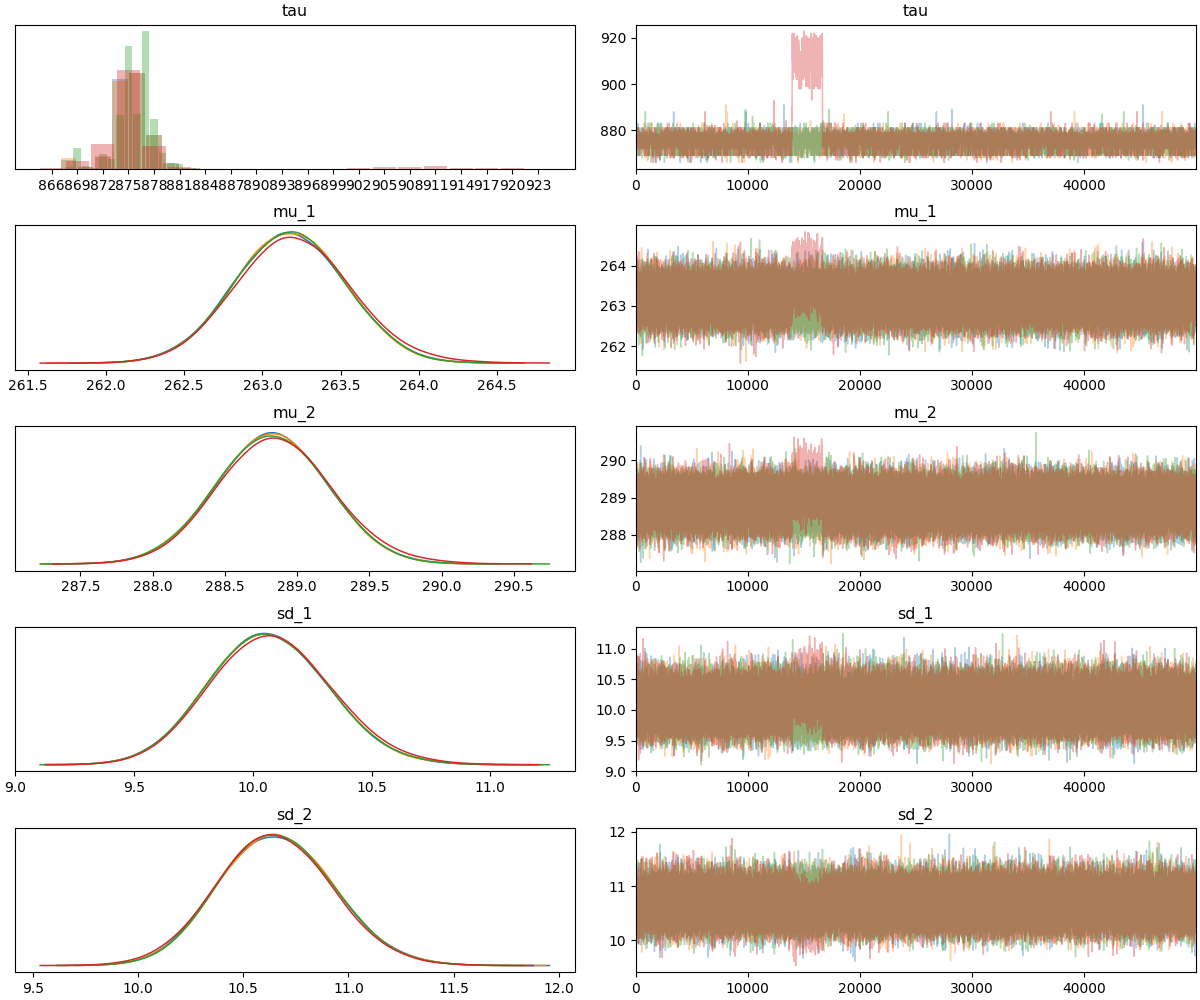
\includegraphics[scale=0.6]{driving-distance-pymc3-posteriors.png}\\
    Figure 2: Posterior traces for each parameter. Each parameter is sampled via four traces. Traces overlap very well for each parameter, indicating soundness of the model and the convergence of the sampler. Of note is the bimodality of $\tau$. The sampler appears to have captured the second switchpoint as well as the first, albeit with some degree of difficulty given the relatively small amplitude of the second switchpoint samples.
\end{center}



\end{document}
